%%%%%%%%%%%%%%%%%%%%%%%%%%%%%%%%%%%%%%%%%
% Journal Article
% Advanced Computer Network
% Practical 6: Submit here the topology snap, output of the commands showing the proper configurations of the WFQ and MQC class based WFQ  experiment. Submit your topology files as well. Total two files to be submitted, topology file in GNS3 and output with necessary screens
%
% Gahan M. Saraiya
% 18MCEC10
%
%%%%%%%%%%%%%%%%%%%%%%%%%%%%%%%%%%%%%%%%%
%----------------------------------------------------------------------------------------
%       PACKAGES AND OTHER DOCUMENT CONFIGURATIONS
%----------------------------------------------------------------------------------------
\documentclass[paper=letter, fontsize=12pt]{article}
\usepackage[english]{babel} % English language/hyphenation
\usepackage{amsmath,amsfonts,amsthm} % Math packages
\usepackage[utf8]{inputenc}
\usepackage{float}

\usepackage{lipsum} % Package to generate dummy text throughout this template
\usepackage{blindtext}
\usepackage{graphicx} 
\usepackage{caption}
\usepackage{subcaption}
\usepackage[sc]{mathpazo} % Use the Palatino font
\usepackage[T1]{fontenc} % Use 8-bit encoding that has 256 glyphs
\usepackage{bbding}  % to use custom itemize font
\linespread{1.05} % Line spacing - Palatino needs more space between lines
\usepackage{microtype} % Slightly tweak font spacing for aesthetics
\usepackage[hmarginratio=1:1,top=32mm,columnsep=20pt]{geometry} % Document margins
\usepackage{multicol} % Used for the two-column layout of the document
%\usepackage[hang, small,labelfont=bf,up,textfont=it,up]{caption} % Custom captions under/above floats in tables or figures
\usepackage{booktabs} % Horizontal rules in tables
\usepackage{float} % Required for tables and figures in the multi-column environment - they need to be placed in specific locations with the [H] (e.g. \begin{table}[H])
\usepackage{hyperref} % For hyperlinks in the PDF
\usepackage{lettrine} % The lettrine is the first enlarged letter at the beginning of the text
\usepackage{paralist} % Used for the compactitem environment which makes bullet points with less space between them
\usepackage{abstract} % Allows abstract customization
\renewcommand{\abstractnamefont}{\normalfont\bfseries} % Set the "Abstract" text to bold
\renewcommand{\abstracttextfont}{\normalfont\small\itshape} % Set the abstract itself to small italic text
\usepackage{titlesec} % Allows customization of titles

\renewcommand\thesection{\Roman{section}} % Roman numerals for the sections
\renewcommand\thesubsection{\Roman{subsection}} % Roman numerals for subsections

\titleformat{\section}[block]{\large\scshape\centering}{\thesection.}{1em}{} % Change the look of the section titles
\titleformat{\subsection}[block]{\large}{\thesubsection.}{1em}{} % Change the look of the section titles
\newcommand{\horrule}[1]{\rule{\linewidth}{#1}} % Create horizontal rule command with 1 argument of height
\usepackage{fancyhdr} % Headers and footers
\pagestyle{fancy} % All pages have headers and footers
\fancyhead{} % Blank out the default header
\fancyfoot{} % Blank out the default footer

\fancyhead[C]{Institute of Technology, Nirma University $\bullet$ October 2018} % Custom header text

\fancyfoot[RO,LE]{\thepage} % Custom footer text
%----------------------------------------------------------------------------------------
%       TITLE SECTION
%----------------------------------------------------------------------------------------
\title{\vspace{-15mm}\fontsize{24pt}{10pt}\selectfont\textbf{Practical 6: Configure WFQ based on topology in GNS3}} % Article title
\author{
\large
{\textsc{Gahan Saraiya, 18MCEC10 }}\\[2mm]
%\thanks{A thank you or further information}\\ % Your name
\normalsize \href{mailto:18mcec10@nirmauni.ac.in}{18mcec10@nirmauni.ac.in}\\[2mm] % Your email address
}
\date{}
\hypersetup{
	colorlinks=true,
	linkcolor=blue,
	filecolor=magenta,      
	urlcolor=cyan,
	pdfauthor={Gahan Saraiya},
	pdfcreator={Gahan Saraiya},
	pdfproducer={Gahan Saraiya},
}
%----------------------------------------------------------------------------------------
\usepackage[utf8]{inputenc}
\usepackage[english]{babel}
\usepackage[utf8]{inputenc}
\usepackage{fourier} 
\usepackage{array}
\usepackage{makecell}

\renewcommand\theadalign{bc}
\renewcommand\theadfont{\bfseries}
\renewcommand\theadgape{\Gape[4pt]}
\renewcommand\cellgape{\Gape[4pt]}
\newcommand*\tick{\item[\Checkmark]}
\newcommand*\arrow{\item[$\Rightarrow$]}
\newcommand*\fail{\item[\XSolidBrush]}
\usepackage{xcolor}
\usepackage{minted} % for highlighting code sytax

\definecolor{LightGray}{gray}{0.9}

\setminted[text]{
	baselinestretch=1.2,
	bgcolor=LightGray,
	fontsize=\small
}

\setminted[sh]{
	baselinestretch=1.2,
	bgcolor=LightGray,
	fontsize=\small
}
\begin{document}
\maketitle % Insert title
\thispagestyle{fancy} % All pages have headers and footers


\section{Introduction}
\paragraph{} Aim of this practical is to Configure \href{https://www.cisco.com/en/US/docs/ios/12_0t/12_0t5/feature/guide/cbwfq.html}{WFQ} on the ethernet 0/1 interface of router R2. The output hold-queue size should be 128, length of 16 for congestive discard threshold, a maximum of 128 conversations and 4 queues for RSVP.


\section{Configuration}
Below steps are to be followed in order to initially configure IP address of router.
Here Below are the configuration taken for configuring routers.

%\begin{table}[H]
%	\centering
%	\bgroup
%	\setlength{\parindent}{-5em} 
%	\caption*{Comparitive analysis}
%	\begin{tabular}{r | c | c | c | c }
%		\textbf{Router} & \textbf{linked to} & \textbf{Interface} & \textbf{IP address} & \textbf{Subnet}\\
%		\hline
%		\hline
%		R1 (AS 100) & 
%		\makecell[l]{
%			R2
%			\\ R3
%		} & 
%		\makecell[l]{
%			Ethernet 1/1
%			\\ Ethernet 1/2
%		} & 
%		\makecell[l]{
%			192.168.12.1
%			\\ 192.168.13.1
%		} & 
%		\makecell[l]{
%			255.255.255.0
%			\\ 255.255.255.0
%		}
%		\\
%		\hline
%		R2 (AS 200) & 
%		\makecell[l]{
%			R1
%		} & 
%		\makecell[l]{
%			Ethernet 1/1
%		} & 
%		\makecell[l]{
%			192.168.12.2
%		} & 
%		\makecell[l]{
%			255.255.255.0
%		}
%		\\
%		\hline
%		R3 (AS 300) & 
%		\makecell[l]{
%			R1
%		} & 
%		\makecell[l]{
%			Ethernet 1/2
%		} & 
%		\makecell[l]{
%			192.168.13.3
%		} & 
%		\makecell[l]{
%			255.255.255.0
%		}
%	\end{tabular}
%	\egroup
%\end{table}

\subsection{Setup WFQ}

\subsubsection{Enter to configuration mode}
\begin{minted}{sh}
R1#conf t
\end{minted}

\subsubsection{Select interface to Configure WFQ}
\begin{minted}{sh}
R1(config)#int ethernet0/1
\end{minted}

\subsubsection{Set interface `up` - make active}
\begin{minted}{sh}
R1(config-if)#no shut
\end{minted}

\subsubsection{set bandwidth to 64 kbps}
\begin{minted}{sh}
R1(config-if)#bandwidth 64
\end{minted}

\subsubsection{Set fair queue}
\begin{minted}{sh}
R1(config-if)#fair-queue 16 128 4
\end{minted}
above command can be interpreted as:
\begin{minted}[breaklines]{text}
fair-queue <congestive-discard-threshold> <number-dynamic-conversation-queue> <number-reservable-conversation-queue>
\end{minted}

\subsection{Set output hold-queue}
\begin{minted}{sh}
R1(config-if)#hold-queue 128 out
\end{minted}

\begin{figure}[H]
	\setlength{\parindent}{-5em} 
	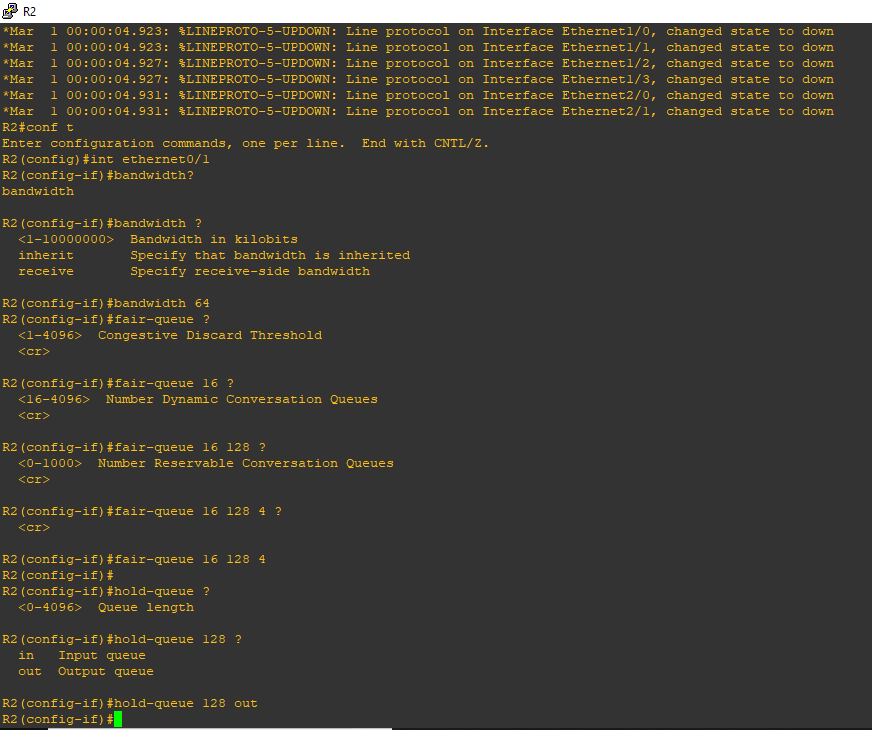
\includegraphics[width=550px]{refs/1}
	\caption{WFQ setup}
\end{figure}

\subsection{Configure the hardware queue on router}
\begin{minted}{sh}
R1(config-if)#tx-ring-limit 1
\end{minted}

\begin{figure}[H]
	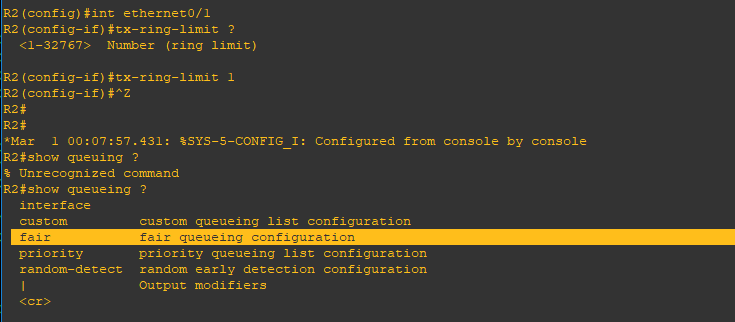
\includegraphics[width=450px]{refs/hardware}
	\caption{Configured the hardware queue on router}
\end{figure}

\subsubsection{Write configuration}
\begin{minted}{sh}
R1#wr
\end{minted}


\subsubsection{check status}
\begin{minted}{sh}
R1#show queueing interface e0/1
\end{minted}

\begin{figure}[H]
	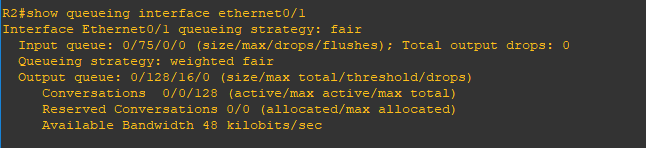
\includegraphics[width=450px]{refs/sh-status}
	\caption{Configuration status \\figure shows available bandwidth is 48 Kbps which is 75\% of total 64Kbps}
\end{figure}



\subsection{Setup CBWFQ}
Aim of this task is to st up class based WFQ on router with outbound Policy described below:
\begin{itemize}
	\item HTTP traffic should get a bandwidth of 16Kbps and the queue should have a maximum of 12 packets.
	\item RTP traffic should get a bandwidth of 96Kbps and the queue should have a maximum of 32 packets.
\end{itemize}

\subsubsection{Step 1}
\begin{itemize}
	\item Enter configuration mode
\begin{minted}{sh}
R1#conf t
\end{minted}
	
	\item Select interface to Configure CBWFQ
\begin{minted}{sh}
R1(config)#int ethernet0/0
\end{minted}
	
	\item set bandwidth to 128 kbps
\begin{minted}{sh}
R1(config-if)#bandwidth 128
\end{minted}

	\item creating the class map HTTP and policy map CBWFQ
\begin{minted}{sh}
R1(config)#class-map HTTP
R1(config-cmap)#match protocol http
R1(config-cmap)#exit
R1(config)#class-map RTP
R1(config-cmap)#match protocol RTP
R1(config-cmap)#exit
R1(config)#class-map TELNET
R1(config-cmap)#match protocol telnet
R1(config-cmap)#exit
R1(config)#policy-map CBWFQ
\end{minted}

	\item Limit HTTP traffic to 16kbps
\begin{minted}{sh}
R1(config-pmap)#class HTTP
R1(config-pmap-c)#bandwidth 16
\end{minted}

	\item Limit HTTP queue to have a maximum of 12 packets
\begin{minted}{sh}
R1(config-pmap)#class HTTP
R1(config-pmap-c)#bandwidth 16
\end{minted}
	\begin{figure}[H]
		\setlength{\parindent}{-5em} 
		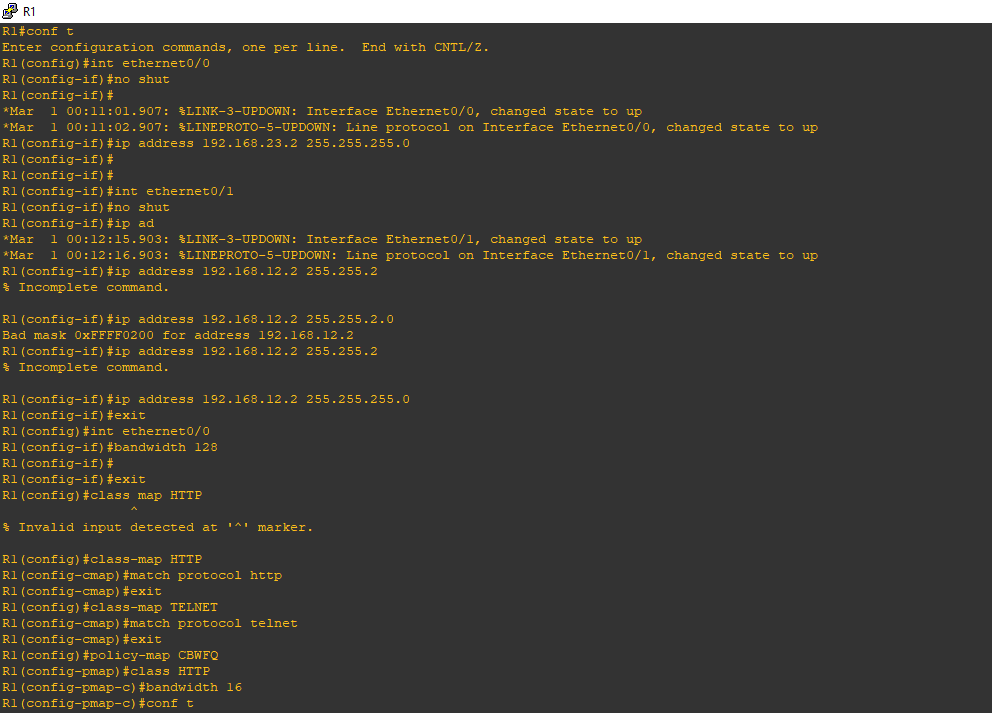
\includegraphics[width=550px]{refs/http-bandwidth.png}
		\caption{Class and policy configuration}
	\end{figure}

	\item Limit HTTP queue to have a maximum of 12 packets
\begin{minted}{sh}
R1(config-pmap)#class HTTP
R1(config-pmap-c)#queue-limit 12
\end{minted}

	\item Configure RTP queue to have a maximum of 32 packets and bandwidth 96kbps
\begin{minted}{sh}
R1(config-pmap)#class HTTP
R1(config-pmap-c)#bandwidth 96
R1(config-pmap-c)#queue-limit 12
\end{minted}
	\begin{figure}[H]
		\setlength{\parindent}{-5em} 
		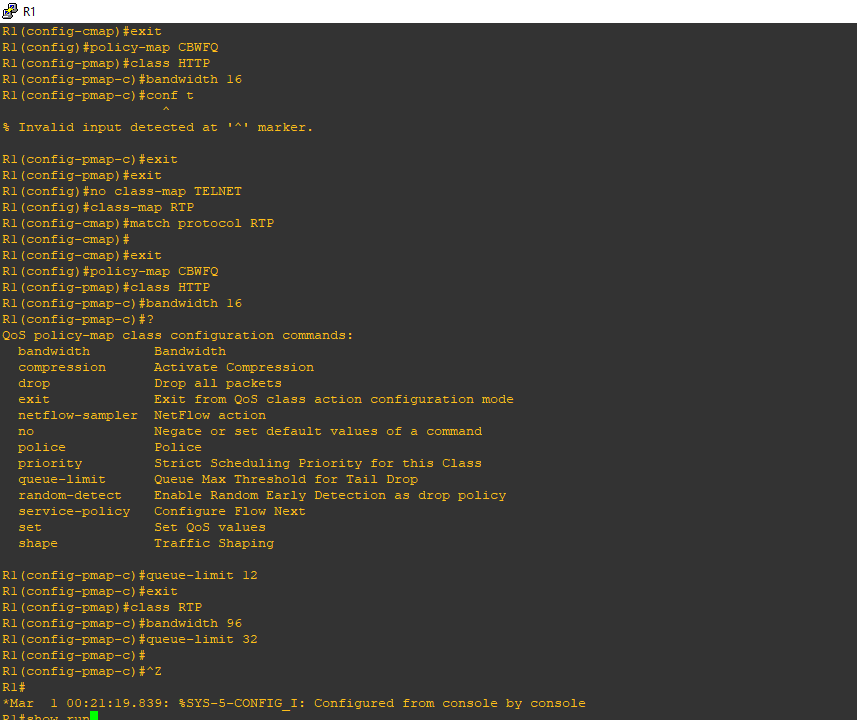
\includegraphics[width=550px]{refs/rtp}
		\caption{configuring bandwidth for traffic policies}
	\end{figure}
\end{itemize}

\begin{figure}[H]
	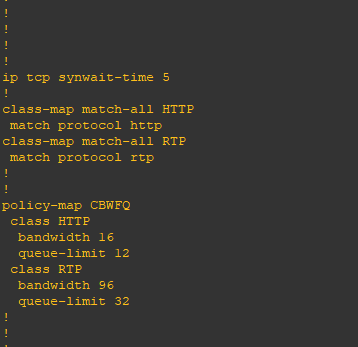
\includegraphics[width=450px]{refs/classmaps}
	\caption{Class maps of system}
\end{figure}

\begin{figure}[H]
	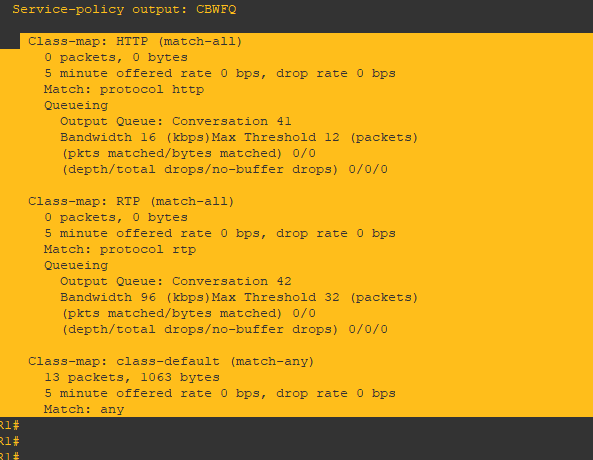
\includegraphics[width=450px]{refs/ex-CBWFQ}
	\caption{Explaining CBWFQ}
\end{figure}


\begin{figure}[H]
	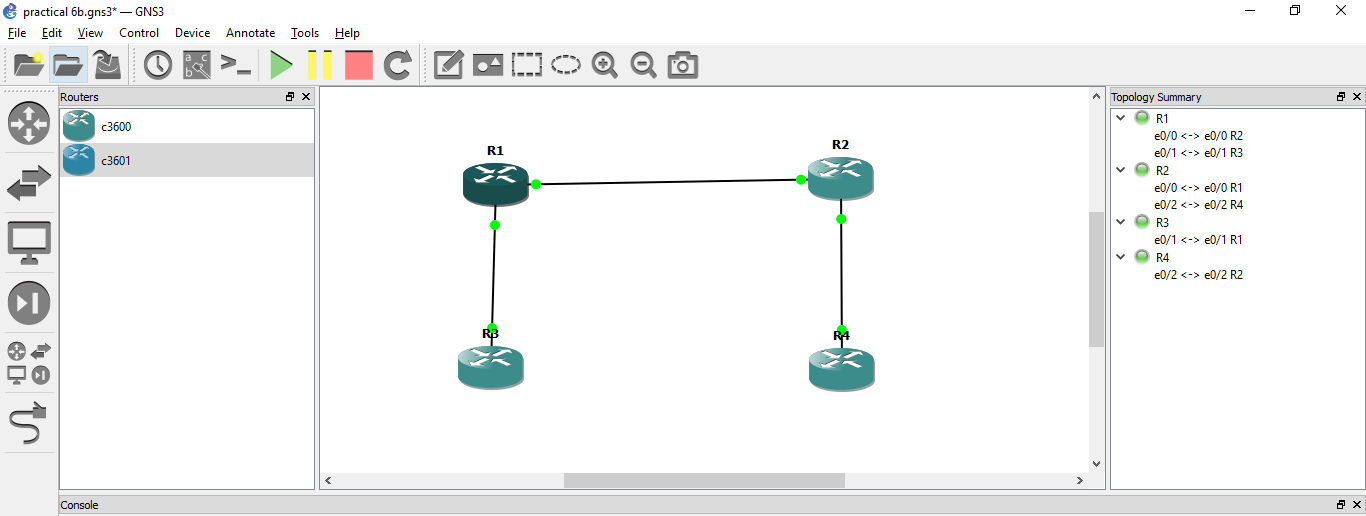
\includegraphics[width=450px]{refs/final_topology}
	\caption{Final topology}
\end{figure}




\end{document}
